%EXP


\begin{figure}[h]
\centering
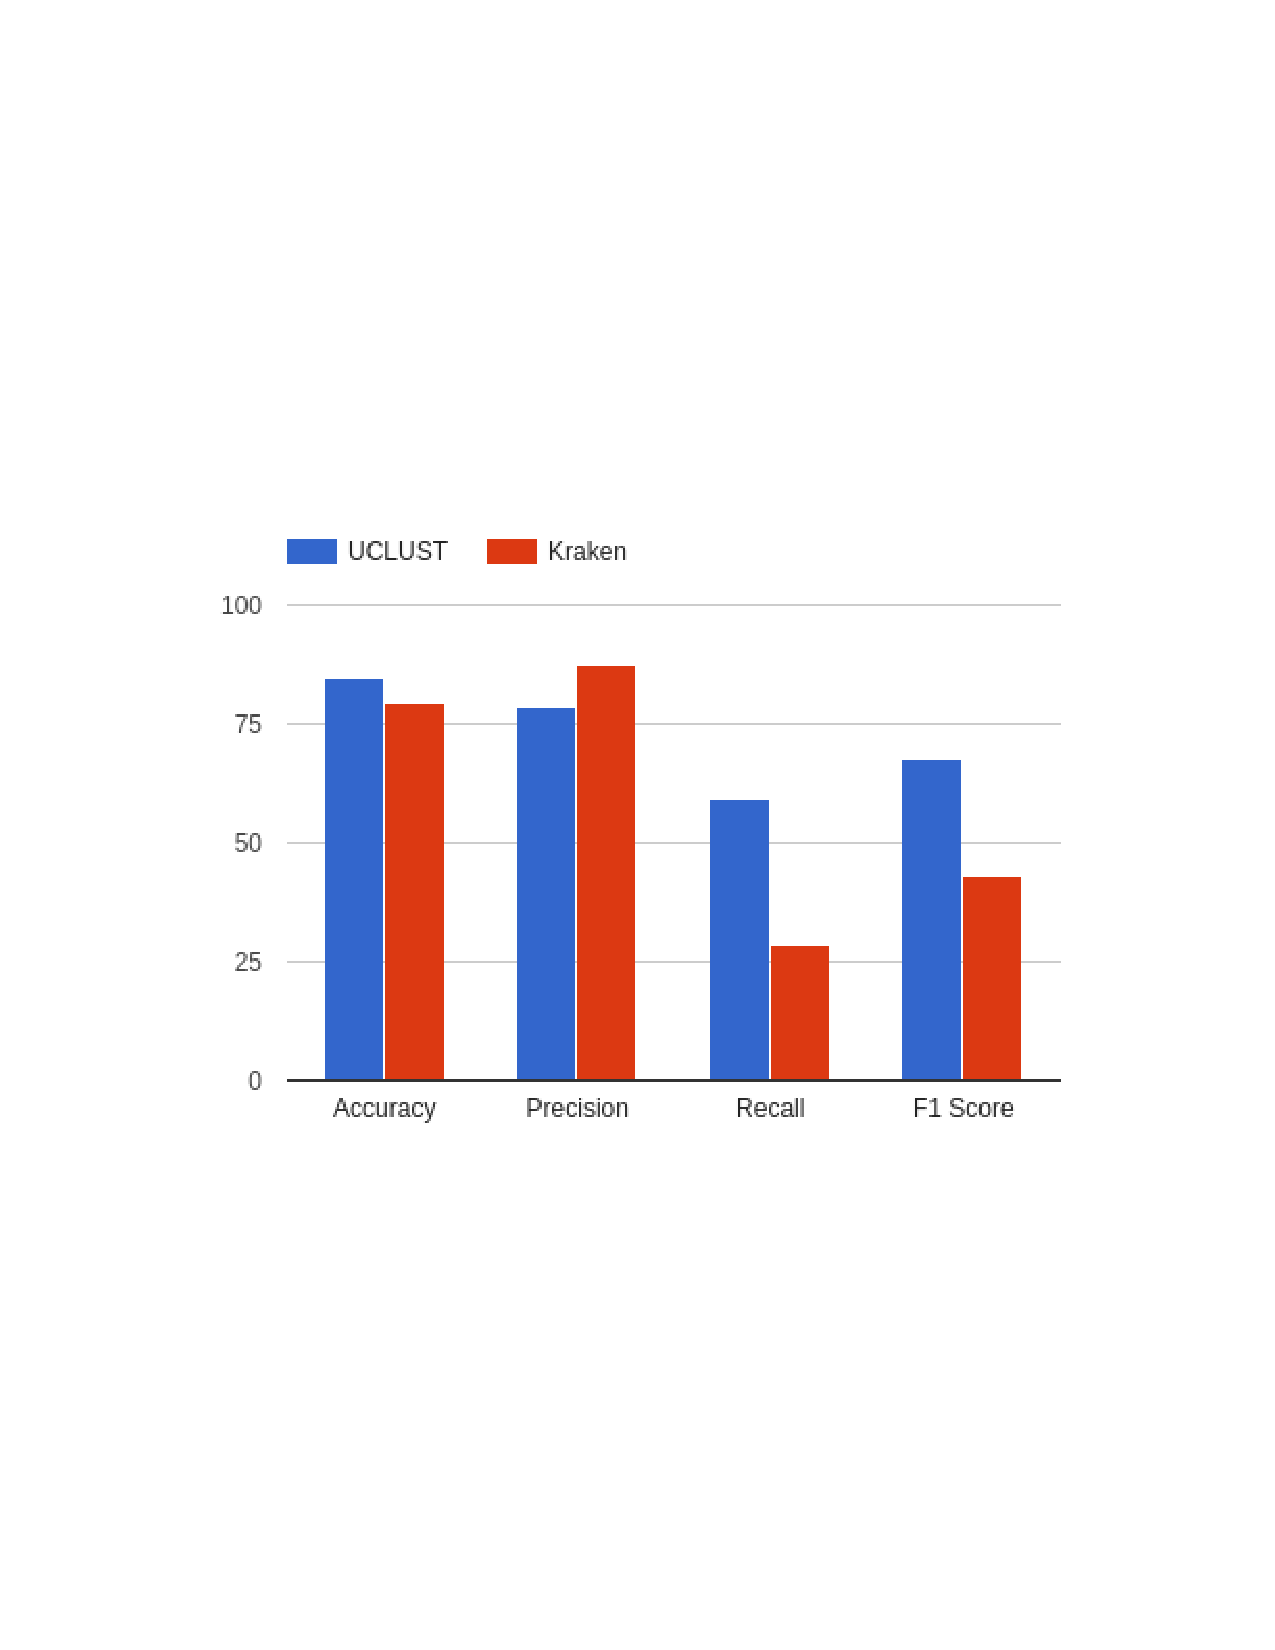
\includegraphics[scale=0.5]{./diagrams/PreFeatEng}
\caption{This diagram shows the results for the comparison between UCLUST and Kraken when classifying "Encephalopathy" versus all other classes. UCLUST had an accuracy and F1-Score of 84.53\% and 67.44\% respectively. Kraken didn't perform as well, with an accuracy of 79.56\% and an F1-Score of 43.08\%. \label{prefeature}}
\end{figure}

\begin{table*}[t]
\begin{center}
\caption{Comparative Run Time of UCLUST and Kraken Representations. \label{tab:time}}
\begin{tabular}{|c|c|}\hline
Representation & Time\\\hline
UCLUST & 180s\\\hline
Kraken & 120s\\\hline
\end{tabular}
\end{center}
\end{table*}


\begin{table*}[t]
\begin{center}
\caption{Comparative Performance of UCLUST and Kraken Representations. 
\label{tab:comp}}
\begin{tabular}{|c|cccc|cccc|}\hline
Representation & Accuracy & Precision & Recall & F1-Score & LOOCV Accuracy & LOOCV Precision & LOOCV Recall & LOOCV F1-Score\\\hline
UCLUST & 84.53 & 78.38 & 59.18 & 67.44 & 88.26 & 83.22 & 67.39 & 74.47\\\hline
Kraken & 79.56 & 87.5 & 28.57 & 43.08 & 78.18 & 70.31 & 24.46 & 36.29\\\hline
\end{tabular}
\end{center}
\end{table*}


\begin{table*}[t]
\begin{center}
\caption{Three Pairwise Comparisons Using UCLUST. \label{tab:pairuclust}}
\begin{tabular}{|c|cccc|cccc|}\hline
Comparison & Accuracy & Precision & Recall & F1-Score & LOOCV Accuracy & LOOCV Precision & LOOCV Recall & LOOCV F1-Score\\\hline
Encephalopathy vs. No Encephalopathy & 88.68 & 90 & 86.54 & 88.23 & 84.47 & 81.77 & 81.77 & 81.77\\\hline
Encephalopathy vs. Control & 96.72 & 95.35 & 100 & 97.62 & 94.26 & 93.2 & 100 & 96.48\\\hline
No Encephalopathy vs. Control & 83.78 & 82.61 & 100 & 90.48 & 87.5 & 86.96 & 99.59 & 92.85\\\hline
\end{tabular}
\end{center}
\end{table*}


\begin{table*}[t]
\begin{center}
\caption{Three Pairwise Comparisons Using Kraken. \label{tab:pairkraken}}
\begin{tabular}{|c|cccc|cccc|}\hline
Comparison & Accuracy & Precision & Recall & F1-Score & LOOCV Accuracy & LOOCV Precision & LOOCV Recall & LOOCV F1-Score\\\hline
Encephalopathy vs. No Encephalopathy & 67.92 & 82.14 & 44.23 & 57.50 & 68.94 & 72.07 & 44.20 & 54.79\\\hline
Encephalopathy vs. Control & 78.69 & 76.92 & 97.56 & 86.02 & 79.51 & 81.14 & 96.35 & 88.09\\\hline
No Encephalopathy vs. Control & 77.03 & 77.03 & 100 & 87.02 & 81.42 & 81.42 & 100 & 89.76\\\hline
\end{tabular}
\end{center}
\end{table*}


\begin{table*}[t]
\begin{center}
\caption{Comparative Performance After Feature Engineering. \label{tab:pfe}}
\begin{tabular}{|c|cccc|cccc|}\hline
Representation & Accuracy & Precision & Recall & F1-Score & LOOCV Accuracy & LOOCV Precision & LOOCV Recall & LOOCV F1-Score\\\hline
UCLUST & 85.64 & 79.49 & 63.27 & 70.46 & 88.54 & 82.58 & 69.57 & 75.52\\\hline
Kraken & 80.66 & 76.92 & 40.82 & 53.34 & 80.8 & 75.86 & 35.87 & 48.93\\\hline
\end{tabular}
\end{center}
\end{table*}


\begin{table*}[t]
\begin{center}
\caption{Three Pairwise Comparisons Using UCLUST After Feature Engineering. \label{tab:pairuclustfe}}
\begin{tabular}{|c|cccc|cccc|}\hline
Comparison & Accuracy & Precision & Recall & F1-Score & LOOCV Accuracy & LOOCV Precision & LOOCV Recall & LOOCV F1-Score\\\hline
Encephalopathy vs. No Encephalopathy & 88.68 & 90 & 86.54 & 88.23 & 86.35 & 83.24 & 85.08 & 84.15\\\hline
Encephalopathy vs. Control & 96.72 & 95.35 & 100 & 97.62 & 95.08 & 94.12 & 100 & 96.97\\\hline
No Encephalopathy vs. Control & 87.84 & 86.36 & 100 & 92.68 & 91.22 & 90.57 & 99.59 & 95.05\\\hline
\end{tabular}
\end{center}
\end{table*}


\begin{table*}[t]
\begin{center}
\caption{Three Pairwise Comparisons Using Kraken After Feature Engineering. \label{tab:pairkrakenfe}}
\begin{tabular}{|c|cccc|cccc|}\hline
Comparison & Accuracy & Precision & Recall & F1-Score & LOOCV Accuracy & LOOCV Precision & LOOCV Recall & LOOCV F1-Score\\\hline
Encephalopathy vs. No Encephalopathy & 69.81 & 83.33 & 48.08 & 60.98 & 77.18 & 80.88 & 60.77 & 69.40\\\hline
Encephalopathy vs. Control & 86.89 & 86.67 & 95.12 & 90.70 & 87.30 & 88.15 & 96.88 & 92.31\\\hline
No Encephalopathy vs. Control & 77.03 & 77.78 & 98.25 & 86.82 & 82.77 & 82.53 & 100 & 90.43\\\hline
\end{tabular}
\end{center}
\end{table*}


Table \ref{tab:time} shows 
the run time of each representation in seconds. We had total of 1.3 million sequence reads. UCLUST unsupervised clustering 
took 180 seconds, while Kraken's OTU database lookups took 120 seconds.

Figure \ref{prefeature} and Table \ref{tab:comp} show 
the classification performance of UCLUST and 
Kraken in distinguishing patients in the "Encephalopathy" class versus 
the other classes. UCLUST correctly predicted the clinical 
phenotype 84.53\% of the time, and had a precision of 78.38\% and recall of 59.18\% on the held-out set. LOOCV results were 
slightly better for each metric than results on the test 
set by about 4-8\%. Kraken had an accuracy of 79.56\% with an even 
larger disparity between precision and recall (87.5\% for the former and 
28.57\% for the latter), which led to a relatively poor F1-score of 43.08\%. LOOCV results for Kraken 
were worse by 1.38\% for accuracy, 17.19\% for precision, 4.11\% for recall, and 6.79\% for F1-Score. As 
the results show, UCLUST generally performed better as a feature 
representation, with 4.97\% higher accuracy and 24.36\% higher F1-score.

Table \ref{tab:pairuclust} displays the performance of UCLUST-based classification 
with regards to training three one-versus-one clinical phenotypic classifiers.  The first comparison 
distinguished between the "Encephalopathy" class and the "No Encephalopathy" class, effectively determining whether or not a patient who had liver cirrhosis also had encephalopathy. Results were much improved when compared with the findings in table \ref{tab:comp}. The accuracy, precision, recall, and F1-score were all  86-90\%. LOOCV
results were worse by about 4-8\% per metric. The 
second comparison distinguished between the "Encephalopathy" class and 
the "Control" class, effectively determining whether a 
patient had encephalopathy caused by liver cirrhosis or had neither disease. This comparison had the best results of the ones we examined, with greater than 95\% performance in all metrics and 100\% recall. The cross validation
results were about 1-2\% worse for each metric except recall, which was still 100\%. The 
third comparison distinguished between the "No Encephalopathy and liver cirrhosis" class and the "Control" class, effectively determining which among the patients lacking encephalopathy had liver cirrhosis. This comparison had an accuracy of 83.78\% and precision of 82.61\%, but had a 100\% recall which led to a high F1-score of 90.48\%. Cross validation results were better by 3.72\% for accuracy, 4.35\% for precision, and 2.37\% better for F1-Score, with essentially the same recall.  Apart from the accuracy and precision of the third comparison, these three pairwise comparisons generally performed better across the board than the results in Table \ref{tab:comp}, with the second pairwise comparison having the best performance.

Table \ref{tab:pairkraken} displays the performance of Kraken with regards to the same three pairwise comparisons described above. For the Encephalopathy vs. No Encephalopathy run, the accuracy was 67.92\%, with 82.14\% precision, 44.23\% recall, and 57.50\% F1-Score. Cross validation produced a precision that was 10.07\% lower but largely the same accuracy and recall. The Encephalopathy vs. Control run produced good results, with 78.69\% accuracy, 76.92\% precision, 97.56\% recall, and 86.02\% F1-Score. LOOCV results mostly confirmed those results, except the precision, which was 4.22\% higher. The No Encephalopathy vs. Control run had quite similar results to the Encephalopathy vs. Control run. The main pattern that appears to emerge from these results is that the recall for Kraken was generally far superior in the pairwise runs than in the original run, which increased the F1-Scores but resulted in similar accuracy and precision. The Encephalopathy vs. No Encephalopathy run was significantly worse than the other two.

Table \ref{tab:pfe} shows the results for the same setup as 
in Table \ref{tab:comp} after we performed feature engineering. For both representations in Table \ref{tab:comp}, the recall was significantly lower than the precision, indicating that there were many more false negatives than false positives. We thus engineered the features in the training set. Certain features in the training set were most strongly present in positive patients, and as such were correlated with positive examples. Some examples in the test set had slightly lower values for those features, and were thus labelled by the classifier as negative examples, when in reality they were positive. We aimed to influence some of these borderline false negative predictions by lowering the threshold for those positively correlated features that would lead to an example being predicted as positive. In order to reduce the threshold for those positively correlated features, we applied a multiplier of 0.9 to the values of each feature of every positive patient in the training set. This had the effect of causing some previously borderline negative predictions to become positive predictions, primarily reducing the number of false negatives and improving the recall scores, but also positively impacting most other metrics as well.  Attempts to use a multiplier of 
less than 0.9 did not appear to further 
improve the results.

With the multiplier of 0.9 applied to the 
feature values for positive training examples, the recall 
increased by 4.09\% for UCLUST and by 12.25\% for Kraken. This was confirmed in the 
cross validation results as well, 
in which UCLUST's recall increased by 2.18\% and 
Kraken's recall increased by 11.41\%. Because of the improvement 
in recall, both representations also had similarly improved F1-Scores after feature engineering. Accuracy and precision remained generally consistent. 
%
Kraken's LOOCV precision 
increased by 5.55\%. This suggests that Kraken's very high precision was tied to its lack of many positive phenotype predictions in general, resulting in a very low number of false positives. While Kraken improved more than UCLUST did due to feature engineering, UCLUST still performed better in all metrics.

Tables \ref{tab:pairuclustfe} and \ref{tab:pairkrakenfe} display the results after the same feature engineering techniques were applied to the pairwise results in \ref{tab:pairuclust} and \ref{tab:pairkraken}, respectively. UCLUST's No Encephalopathy vs. Control run saw an increase of 4.06\% in accuracy, 3.75\% in precision, and similar gains in its cross validation results for accuracy and precision. UCLUST's other two runs were largely unaffected, albeit with slightly better cross validation results. Kraken's Encephalopathy vs. Control run was greatly improved after feature engineering, with an 8.20\% increase in accuracy and a 9.75\% increase in precision, with similar increases in cross validation results. This more than offset a slight decrease in recall. The Encephalopathy vs. No Encephalopathy run had mostly unchanged results, albeit with much improved cross validation scores, and the No Encephalopathy vs. Control run was not significantly affected.